\begin{appendix}
\section{Matsubara Frequencies and Fast Fourier Transform}
In order to solve the impurity model we have to perform several Fourier Transform.
As we consider electrons, the Green's function in imaginary time is antiperiodic by shifts of $\beta$, so we have to use fermionic Matsubara frequencies $ω_n:=\frac{π(2n+1)}{β}$.
The Fourier Transformations are given by:

\begin{align}
  G(i ω_n) &:= \int_0^β dτ G(τ) e^{i ω_n τ}\\
  G(τ) &= \frac{1}{β} \sum_{i ω_n} G(i ω_n) e^{-i ω_n τ}
\end{align}
For effient calculations we use the FFT-algorithm of the numpy package. Therefore we have to adapt our definitions to the implementation of the numpy library. The numpy library calculates its Fourier Transform by:
\begin{equation}
  A_k = \mathrm{FFT}(a_m) =  \sum_{m=0}^{n-1} a_m \exp\left\{-2\pi i{mk \over n}\right\}
   \qquad k = 0,\ldots,n-1.
\end{equation}
Hence, we discretize the Matsubara Fourier transformation
\begin{align}
  G(i ω_{-n}) &\approx \sum_{k=0}^{N-1} \Delta τ \, G(\Delta τ \, k) \exp{\left(i \frac{π (-2n+1)k}{N}\right)}\\
          &=\frac{\beta}{N} \sum_{k=o}^{N-1} \left( G(\Delta τ \, k)\exp{\left(i π \frac{k}{N}\right)}  \right)  \exp{\left(i \frac{-2 π n k}{N}\right)}\\
	  &= \frac{\beta}{N} \mathrm{FFT}\left( G(\Delta τ \, k)\exp{\left(i π \frac{k}{N}\right)}\right), \label{eq:MFFT}
\end{align}
where $\Delta τ = \frac{\beta}{N}$.
The same can be carried out for the inverse Fourier Tranformations.
\begin{align}
	G(\Delta τ k) &= \frac{N}{β} e^{-i π \frac{k}{N}}\frac{1}{N}\sum_{ω_n}G(i ω_{-n}) e^{i 2π n k/N}\\
	&= \frac{N}{β} e^{-i π \frac{k}{N}}\mathrm{IFFT}(G(iω_{-n})) \label{eq:IMFFT}
\end{align}
\begin{figure}[h]
	\centering
	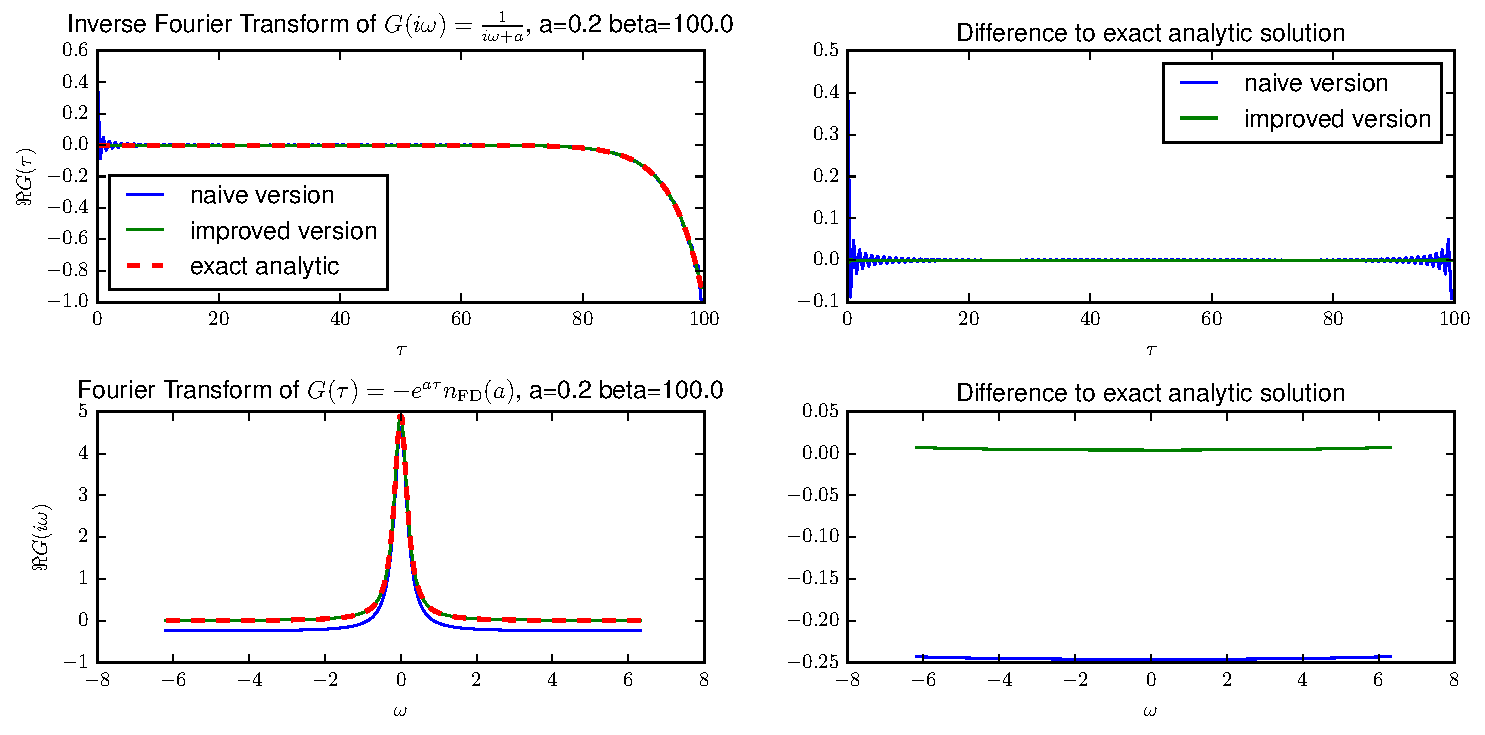
\includegraphics[width=\textwidth]{Matsubara_Fourier_fig}
	\caption{Comparison of the different discretized Fourier Transformations. The improved version, by manually removing the $\frac{1}{i \omega}$ factor, approximates the exact transformation significantly better. }
	\label{fig:fourier_traf}
\end{figure}
Unfortunately the ``naiv'' implementations \eqref{eq:MFFT} and \eqref{eq:IMFFT} cause numerical problems, since a typical Green's function in frequency space is of the form
\begin{equation}
	G(iω_n) = \frac{1}{iω_n +a} = \frac{1}{i ω_n} + \mathcal{O}\left(\frac{1}{ω_n^2}\right).
	\label{eq:expansion}
\end{equation}
Although $a$ can also be frequency dependent, the first term in the expansion of $G$ is always of the form as in \eqref{eq:expansion}.\todo{more details here?} Carrying out the sum over frequencies of this first term does unfortunately not converge, which is why we have to transform the $\frac{1}{i ω_n}$ part manually. %more information here?
From analytical calculation the Fourier transform is given as:
\begin{equation}
	G(τ)=-\frac{1}{2} \quad ⇔ \quad G(i ω_n) =\frac{1}{i ω_n}
	\label{eq:ff_pair}
\end{equation}
Consequently the improved version of our Fourier transformation is given by subtracting and adding the relevant terms before and after the transformation.
\begin{align}
	G(i ω_{-n})&= \frac{1}{i ω_{-n}}+\frac{\beta}{N} \mathrm{FFT}\left( \left(G(\Delta τ \, k)+\frac{1}{2}\right)\exp{\left(i π \frac{k}{N}\right)}\right)\\
	G(\Delta τ k)&= -\frac{1}{2}+\frac{N}{β} e^{-i π \frac{k}{N}}\mathrm{IFFT}\left(G(iω_{-n})-\frac{1}{i ω_{-n}}\right)
	\label{eq:improved_fft}
\end{align}
The improvement can be seen in \figref{fig:fourier_traf}, where we compare the exact Fourier transformation of $G(i ω)=\frac{1}{iω+a}$ to our discretized versions. The naiv version shows significant deviations to the analytic solution, whereas our improved version approximates the exact one very well.  

\section{Pade Approximation}
\todo{Adding Pade approximation}

\end{appendix}
